% ==========================================
% Section 12: Summary & References (Slides 58-62)
% ==========================================

% Slide 58: Summary
\begin{frame}{جمع‌بندی: پیش‌پردازش داده‌ها}
\begin{itemize}
  \item \textbf{داده‌های خام دنیای واقعی همواره با چالش‌های عمده همراهند:}
  \begin{itemize}
    \item مقادیر گمشده و ناتمام (\lr{Missing Values})
    \item خطاها و داده‌های پرت (\lr{Errors \& Outliers})
    \item ابعاد بالا و نفرین ابعاد (\lr{High Dimensionality})
    \item مقیاس‌های ناهمگون و انواع داده‌های پشتیبانی‌نشده
  \end{itemize}
  \vspace{0.3cm}
  \item \textbf{پیش‌پردازش خوب و علمی، پیش‌نیاز حیاتی موفقیت هر پروژه داده‌کاوی است.}
  \begin{itemize}
    \item کیفیت مدل نهایی هرگز نمی‌تواند از کیفیت داده‌های ورودی فراتر رود!
    \item قانون زرین داده‌کاوی: \textbf{\lr{Garbage In, Garbage Out}}
  \end{itemize}
\end{itemize}
\end{frame}

% Slide 59: Prepare Your Data (CrowdFlower Report)
\begin{frame}{آماده‌سازی داده‌ها}
\centering
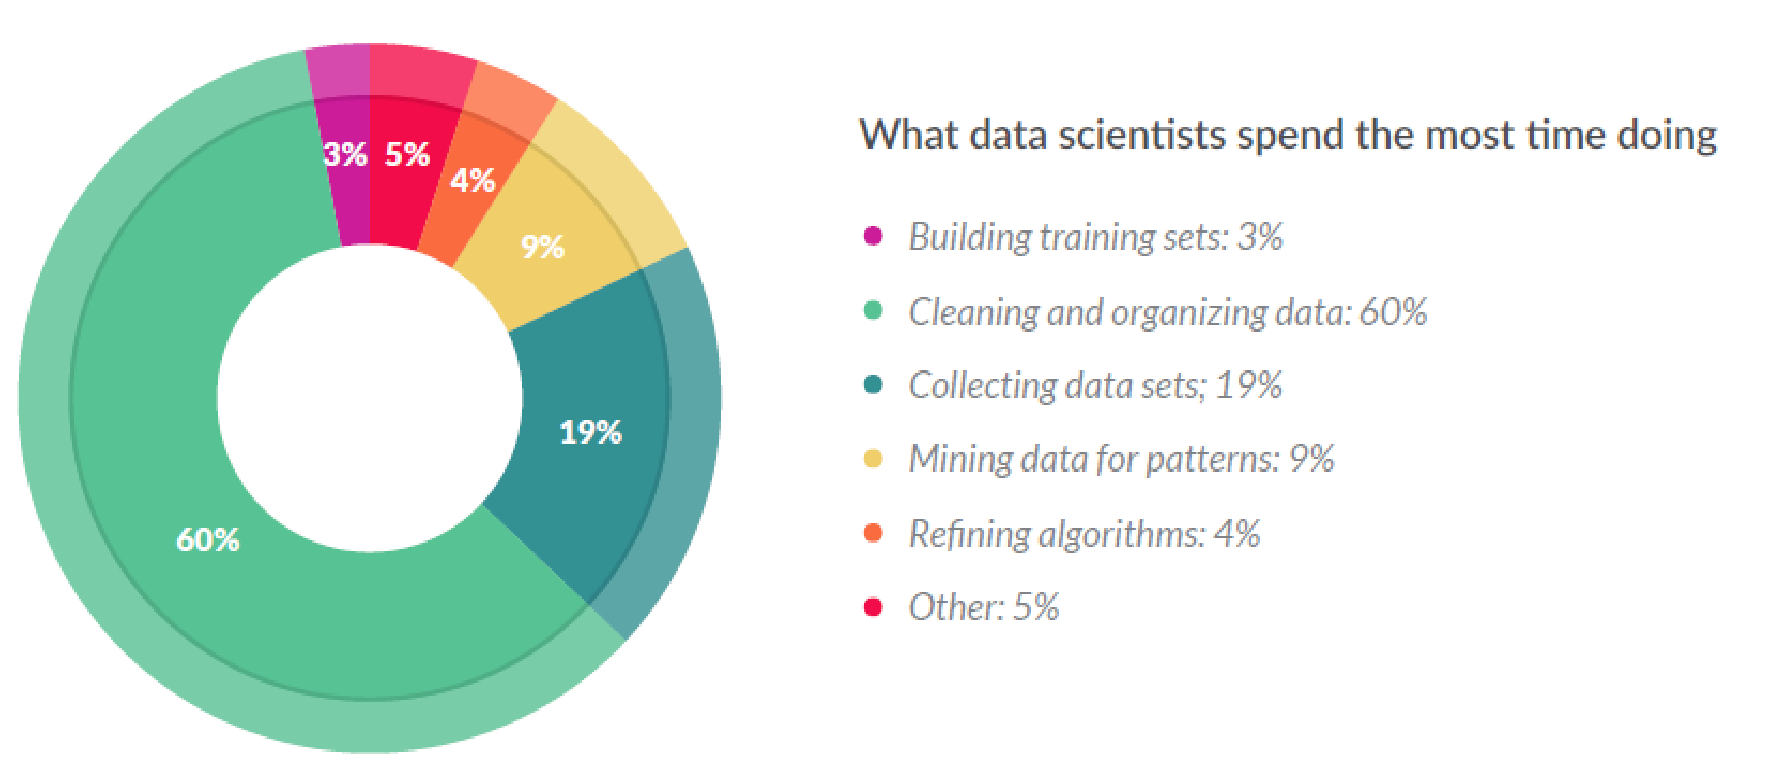
\includegraphics[width=0.88\textwidth]{images/page_59_img_1.png}
\vspace{0.2cm}
\flushright
{\fontsize{6.5}{8}\selectfont\color{subgray}منبع: گزارش علم داده \lr{CrowdFlower 2016} -- \url{http://visit.crowdflower.com/data-science-report.html}}
\end{frame}

% Slide 60: Reminder
\begin{frame}{یادآوری}
\begin{columns}[c]
  \begin{column}{0.55\textwidth}
    \begin{itemize}
      \item \textbf{مطالب ارائه‌شده در کلاس‌های آنلاین:}
      \begin{itemize}
        \item مرتبط با تمرین‌ها و آزمون پایان‌ترم هستند.
      \end{itemize}
    \end{itemize}
  \end{column}
  \begin{column}{0.43\textwidth}
    \centering
    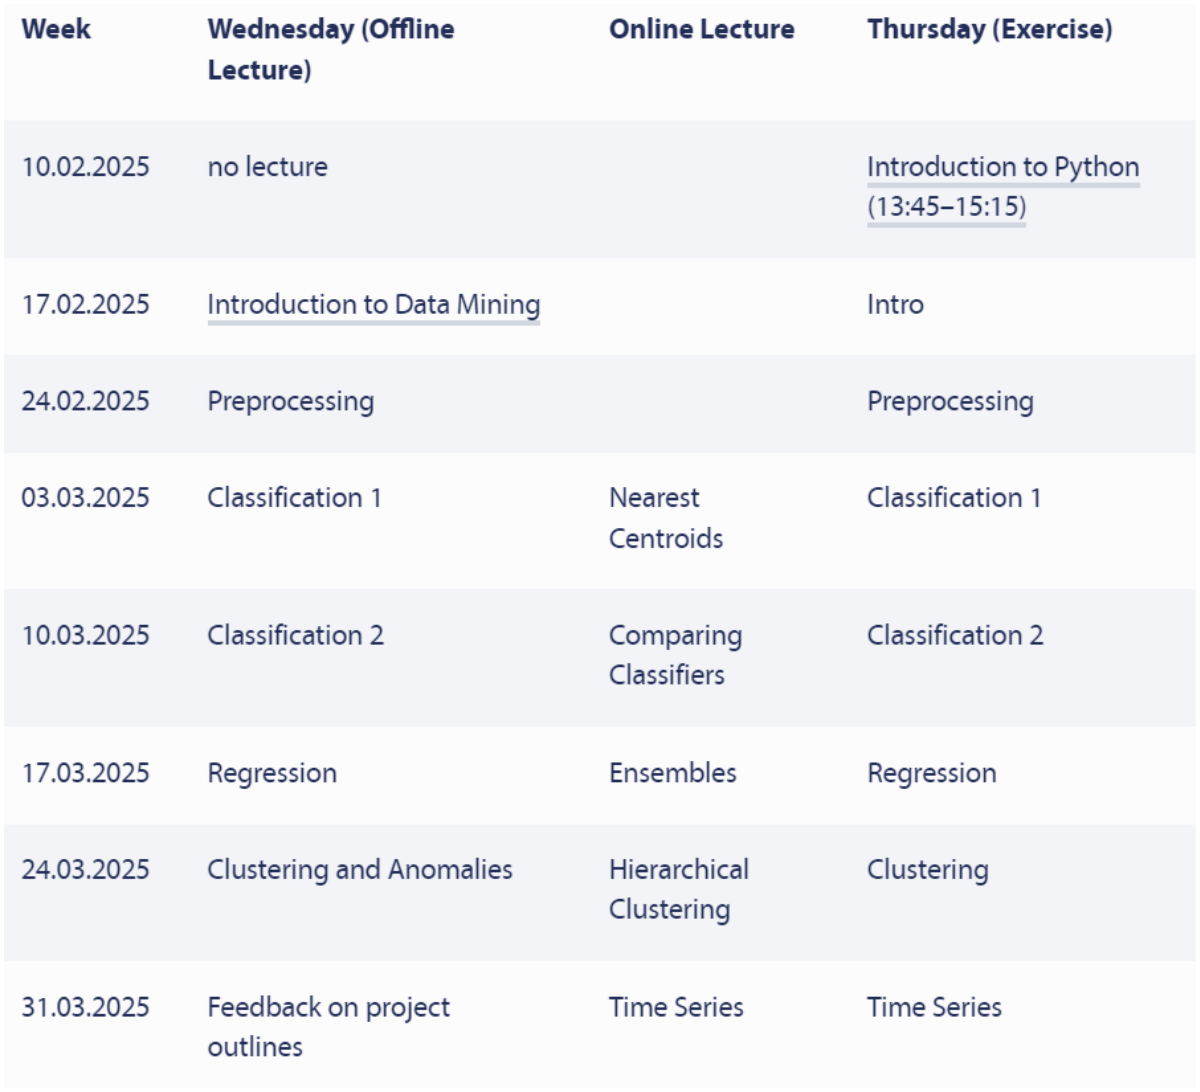
\includegraphics[width=\textwidth]{images/page_60_img_1.png}
  \end{column}
\end{columns}
\end{frame}

% Slide 61: Questions
\begin{frame}{پرسش و پاسخ}
\begin{columns}[c]
  \begin{column}{0.55\textwidth}
    \begin{center}
      {\fontsize{20}{24}\selectfont\color{mannheimblue}\textbf{آیا پرسشی دارید؟}}\\[12pt]
      {\fontsize{11}{14}\selectfont\color{darktext}بحث و تبادل نظر پیرامون مباحث پیش‌پردازش}
    \end{center}
  \end{column}
  \begin{column}{0.43\textwidth}
    \centering
    
\includegraphics[width=\textwidth]{images/page_61_img_1.png}
  \end{column}
\end{columns}
\end{frame}

% Slide 62: Literature
\begin{frame}{منابع و مراجع مطالعاتی برای این اسلایدها}
\begin{itemize}
  \item \textbf{پایتون (\lr{Python}):}
  \begin{itemize}
    \item جایگزینی مقادیر گمشده (\lr{Imputation}):\\
    {\fontsize{7}{9}\selectfont\url{https://scikit-learn.org/1.5/modules/impute.html}}
    \vspace{0.1cm}
    \item پیش‌پردازش (\lr{Preprocessing}):\\
    {\fontsize{7}{9}\selectfont\url{https://scikit-learn.org/1.5/modules/preprocessing.html}}
    \vspace{0.1cm}
    \item استخراج ویژگی از متن (\lr{Text feature extraction}):\\
    {\fontsize{7}{9}\selectfont\url{https://scikit-learn.org/1.5/modules/feature_extraction.html\#text-feature-extraction}}
    \vspace{0.1cm}
    \item انتخاب ویژگی (\lr{Feature Selection}):\\
    {\fontsize{7}{9}\selectfont\url{https://scikit-learn.org/1.5/modules/feature_selection.html}}
  \end{itemize}
\end{itemize}
\end{frame}
